% MCM/ICM 2026 LaTeX 主控文件
% 编译方式:XeLaTeX + Biber(推荐用latexmk自动编译)
% !TEX program = xelatex
% !BIB program = biber

\documentclass{mcmthesis}

% 兼容性补丁:避免旧aux残留的chapter计数器导致hyperref报错
\newcounter{chapter}
\renewcommand{\thechapter}{\arabic{chapter}}

% MCM题目配置(比赛时务必修改tcn为真实队号)
\mcmsetup{
    tcn = {2617892},
    problem = {C},
    sheet = true,
    titleinsheet = true,
    keywordsinsheet = true,
    titlepage = false
}

% 目录开关
\makeatletter
\@ifundefined{showtoctrue}{}{\showtoctrue}
\makeatother

%=== 宏包加载 ===

% 字体与排版
\usepackage{palatino}
\usepackage{microtype}
\setlength{\emergencystretch}{2em}

% 页面与布局
\usepackage{lastpage}
\usepackage{zref-abspage}
\usepackage{float}
\usepackage{geometry}
\setlength{\headheight}{15pt}

% 数学公式
\usepackage{amsmath, amssymb, amsthm}
\usepackage{mathtools}

% 表格美化
\usepackage{booktabs}
\usepackage{tabularx}
\usepackage{longtable}
\usepackage{multirow}
\usepackage{array}
\usepackage{threeparttable}

% 算法伪代码(顶会风格)
\usepackage[ruled, vlined, linesnumbered]{algorithm2e}
\SetAlgorithmName{Algorithm}{algorithm}{List of Algorithms}
\SetKwInput{KwIn}{Input}
\SetKwInput{KwOut}{Output}
\SetKwInput{KwData}{Data}
\SetKwInput{KwResult}{Result}

% 代码高亮
\usepackage{listings}
\lstset{
    basicstyle=\small\ttfamily,
    keywordstyle=\color{blue},
    commentstyle=\color{gray},
    numbers=left,
    numberstyle=\tiny\color{gray},
    frame=single,
    breaklines=true,
    tabsize=4
}

% 图形与颜色
\usepackage{graphicx}
\usepackage{subcaption}
\usepackage{xcolor}
\usepackage{tikz}
\usetikzlibrary{shapes, arrows, positioning, calc}

% 列表与枚举
\usepackage{enumitem}
\setlist[enumerate]{itemsep=0pt, parsep=0pt}

% 彩色框(用于重点内容)
\usepackage{tcolorbox}
\tcbuselibrary{skins, breakable}

% 超链接(最后加载)
\usepackage{hyperref}
\hypersetup{
    colorlinks=true,
    linkcolor=black,
    citecolor=green!50!black,
    urlcolor=blue!80!black
}

% 目录格式调整(紧凑行距)
\usepackage{tocloft}
\setlength{\cftbeforesecskip}{2pt}
\setlength{\cftbeforesubsecskip}{1pt}

% 参考文献
\usepackage[backend=biber, style=ieee, sorting=none]{biblatex}
\addbibresource{ref.bib}

%=== 自定义命令 ===

% 正文页数计数器(实现 Page X of Y)
\newcounter{mainpages}
\makeatletter
\newcommand{\savemainpages}{%
    \immediate\write\@auxout{\string\setcounter{mainpages}{\the\value{page}}}%
}
\makeatother

% 快捷引用命令
\newcommand{\figref}[1]{Fig.~\ref{#1}}
\newcommand{\tabref}[1]{Table~\ref{#1}}
\newcommand{\eqnref}[1]{Eq.~(\ref{#1})}
\newcommand{\algref}[1]{Algorithm~\ref{#1}}
\newcommand{\secref}[1]{Section~\ref{#1}}

%=== 文档元信息 ===

\title{Inferring Fan Votes from Elimination Data: \\ 
       A Dual-Core Inversion Framework with Anomaly Detection \\
       and Mechanism Design for \emph{Dancing with the Stars}}
\author{Team \#2617892}

%=== 正文开始 ===
\begin{document}

% Summary Sheet(摘要页,不计入页数)
\pagenumbering{arabic}
\setcounter{page}{0}
\pagestyle{empty}
\begin{abstract}%以下是25年C题的参考Abstract
    
To ensure a systematic and multidimensional approach to Olympic medal prediction, this study constructs a dynamic and coupled comprehensive \textbf{Predictive Framework}. This framework integrates various objectives, including medal distribution prediction, breakthrough country identification, event performance evaluation, and the impact analysis of coaching resource allocation. By employing multi-source heterogeneous data fusion and machine learning integration methods, we achieve an in-depth analysis and reliable prediction of the development patterns in competitive sports.

First, we develop a multidimensional predictive model to analyze Olympic medal patterns. Utilizing \textbf{Principal Component Analysis (PCA)} for dimensionality reduction and noise filtering of the Olympic event dataset, we combine \textbf{Long Short-Term Memory (LSTM)} networks to mine temporal features and integrate home advantage effects. A dual-channel \textbf{XGBoost-Bootstrap} model is established to generate predictions with a 95\% confidence interval. The results indicate an upward trend for countries such as the United States and the United Kingdom, while countries like France and China show a decline. The model exhibites a high accuracy with a low \textbf{MAE} and \textbf{MAPE}, demonstrating strong robustness. Through non-parametric testing, potential breakthrough countries are identified, with San Marino and Kuwait showing gold medal breakthrough probabilities of \textbf{84.7\%} and \textbf{68.4\%}, respectively.

Subsequently, we develop a \textbf{Difference-in-Differences (DID)} model to quantify the competitive benefits of coaching replacement and conduct statistical significance tests as well as parallel trends tests to ensure the reliability of our results. It is found that during the 2020-2024 period, Australia, South Korea, and Poland experienced significant "great coach" policy effects through strategic restructuring of their coaching teams. Based on this, we recommend prioritizing investment in high-elasticity projects. \textbf{SHapley Additive exPlanations (SHAP)} is further utilized to quantify event contributions, revealing that swimming and athletics serve as core contributing events to medal augmentation.

Furthermore, we explore the potential of a country to win its first-ever medal by constructing a \textbf{Hurdle-Tobit} fusion model. This model addresses the zero-inflation characteristics and heterogeneity between countries. The prediction results show that countries like Angola and Bangladesh have a probability of winning their first medal exceeding \textbf{45\%} in the next Games. Finally, we propose a strategic resource allocation plan using \textbf{Multiobjective Optimization} to balance the "depth" and "breadth" of National Olympic Committees (NOCs), suggesting that high-potential NOCs should prioritize multinational coach introductions in wrestling and table tennis.

In conclusion, our integrated framework synthesizes all models and analyses to present new insights and corresponding decision supports for the global sports community.

\begin{keywords}
    Olympic Medal Prediction, PCA-LSTM, XGBoost, DID Model, Hurdle-Tobit, SHAP Analysis.
\end{keywords}

\end{abstract}

\maketitle
\thispagestyle{empty}

% Memo to DWTS Director(备忘录,紧随摘要页)
% Memo: Transparency Protocol Recommendation

\newpage
\thispagestyle{empty}

\begin{center}
\Large\textbf{MEMORANDUM}
\end{center}

\vspace{0.5em}
\noindent\rule{\textwidth}{1.5pt}
\vspace{0.3em}

\begin{tabular}{@{}ll}
\textbf{TO:}      & Director of Programming, \emph{Dancing with the Stars} \\
\textbf{FROM:}    & Team \#2617892, Data Analytics Consultants \\
\textbf{DATE:}    & January 26, 2026 \\
\textbf{SUBJECT:} & \textbf{Balancing Entertainment and Fairness: A Transparency Protocol}
\end{tabular}

\vspace{0.3em}
\noindent\rule{\textwidth}{1.5pt}
\vspace{0.8em}

\subsection*{Executive Summary}

We commend the Judges' Save rule (introduced S28) for increasing dramatic tension and giving judges meaningful agency. However, our analysis reveals \textbf{model-data mismatches} in S32--S33 that warrant attention---not as evidence of wrongdoing, but as opportunities for improved transparency.

\subsection*{Key Findings}

\begin{itemize}[itemsep=0.1em]
    \item \textbf{S1--S31:} Our LP/MILP model achieves $S^* = 0$ (full consistency with voting rules).
    \item \textbf{S32--S33:} Constraint slack $S^* > 0$ indicates outcomes our model cannot fully explain.
    \item \textbf{Bobby Bones (S27):} Wide survival intervals ($[1\%, 91\%]$) demonstrate how the 50/50 system can protect low-scoring contestants with strong fan bases.
\end{itemize}

\noindent Possible causes for S32--33 mismatches: (1) subjective judge save criteria, (2) bottom-two selection mechanics, (3) multi-dance score aggregation.

\subsection*{Recommendations: Tiered Transparency System}

\begin{enumerate}[itemsep=0.2em]
    \item \textbf{Weighted Percent Scoring:} Adopt $0.6 \times \text{JudgePct} + 0.4 \times \text{FanPct}$. Marketing message: ``60\% skill, 40\% popularity.'' Simulations show \textbf{92.5\% reduction} in wrongful eliminations while preserving fan engagement.
    
    \item \textbf{Judge Save Transparency:} Document and announce criteria for judge save decisions (e.g., ``technical improvement shown'' or ``cumulative season performance''). This reduces perceived arbitrariness.
    
    \item \textbf{Pre-Broadcast Audit (Internal):} Run LP solver before results announcement ($<5$ sec). Flag episodes with $S^* > 0.5$ for producer review---not to change outcomes, but to prepare explanations if questioned.
\end{enumerate}

\subsection*{Why This Matters}

The Judges' Save adds suspense and rewards quality---both valuable for entertainment. Our recommendations \emph{enhance} this by making the save more defensible and the overall system more transparent. Viewers who understand the scoring are more invested, not less.

\vspace{0.5em}
\hfill\textbf{--- Team \#2617892}


% Contents(目录页,从第1页开始但不显示页码)
\newpage
\setcounter{page}{1}
\pagestyle{empty}
\tableofcontents
\thispagestyle{empty}

% 正文开始(从第3页开始显示页眉页码)
\newpage
\setcounter{page}{3}
\pagestyle{fancy}
\fancyhf{}
\fancyhead[L]{\small Team \#2617892}
\fancyhead[R]{\small Page \thepage\ of \themainpages}
\fancyfoot[C]{}

% Section 1: Introduction
% Section 1: Introduction
% 引言:问题背景 + 问题重述 + 利益相关者 + 本文工作

\section{Introduction}
\label{sec:intro}

%=== 1.1 问题背景:强调可持续性挑战 ===
\subsection{Problem Background}
\label{subsec:background}

% 【写作指导】E题引言需强调:
% 1. 环境问题的紧迫性与全球性
% 2. 多利益相关者的复杂博弈
% 3. 可持续发展的长期视角

The 21st century confronts humanity with unprecedented environmental challenges that demand integrated, systems-oriented solutions. \TODO{Describe the specific environmental context of Problem E, e.g., ecosystem degradation, climate adaptation, resource scarcity, clean energy transition.}

The complexity of this challenge arises from several intertwined factors:

\begin{itemize}[itemsep=0.3em]
    \item \textbf{Interconnected Systems:} Environmental, economic, and social systems are deeply coupled, with interventions in one domain producing cascading effects across others.
    
    \item \textbf{Temporal Dynamics:} Sustainability outcomes unfold over decades, requiring models that capture both short-term trade-offs and long-term equilibria.
    
    \item \textbf{Stakeholder Heterogeneity:} Different actors---governments, industries, communities, and future generations---hold divergent values and objectives that must be reconciled.
    
    \item \textbf{Deep Uncertainty:} Climate variability, technological disruptions, and policy shifts introduce substantial uncertainty into any planning framework.
\end{itemize}

\TODO{Add 1-2 paragraphs with specific statistics and references relevant to the Problem E topic. Cite authoritative sources such as IPCC, UN SDGs, or peer-reviewed literature.}

%=== 1.2 问题重述:精确界定任务 ===
\subsection{Restatement of the Problem}
\label{subsec:restatement}

To address the requirements of the 2026 ICM Problem E, we are tasked with developing a comprehensive analytical framework to:

\begin{enumerate}[itemsep=0.4em]
    \item \textbf{Task 1: \TODO{First Sub-Problem}}
    
    \TODO{Restate the first specific question from Problem E. Example: ``Develop a sustainability indicator system that captures environmental, economic, and social dimensions of [topic].''}
    
    \item \textbf{Task 2: \TODO{Second Sub-Problem}}
    
    \TODO{Restate the second specific question. Example: ``Model the dynamic interactions between [key system components] over a [time horizon].''}
    
    \item \textbf{Task 3: \TODO{Third Sub-Problem}}
    
    \TODO{Restate the third specific question. Example: ``Evaluate alternative policy scenarios and identify optimal intervention strategies.''}
    
    \item \textbf{Task 4: \TODO{Fourth Sub-Problem / Policy Memo}}
    
    \TODO{Restate the policy communication requirement. Example: ``Prepare a concise policy brief for [target decision-maker] summarizing key findings and recommendations.''}
\end{enumerate}

%=== 1.3 利益相关者与目标分析 ===
\subsection{Stakeholders and Objectives}
\label{subsec:stakeholders}

% 【E题核心】利益相关者分析是O奖论文的标志性要素
A sustainability-oriented decision framework must explicitly acknowledge the diverse stakeholders affected by and influencing the system. Table~\ref{tab:stakeholders} maps key stakeholders to their primary objectives and potential conflicts.

\begin{table}[H]
    \centering
    \caption{Stakeholder Analysis Matrix}
    \label{tab:stakeholders}
    \begin{tabularx}{\textwidth}{l X X X}
        \toprule
        \textbf{Stakeholder} & \textbf{Primary Objectives} & \textbf{Constraints} & \textbf{Potential Conflicts} \\
        \midrule
        \TODO{Government} & 
        \TODO{Environmental protection, economic growth, public welfare} & 
        \TODO{Budget limitations, political cycles} & 
        \TODO{Short-term growth vs. long-term sustainability} \\
        \addlinespace[0.5em]
        
        \TODO{Communities} & 
        \TODO{Livelihoods, health, cultural preservation} & 
        \TODO{Limited resources, information asymmetry} & 
        \TODO{Development vs. conservation} \\
        \addlinespace[0.5em]
        
        \TODO{Private Sector} & 
        \TODO{Profitability, market share, compliance} & 
        \TODO{Competition, capital constraints} & 
        \TODO{Cost externalization vs. responsibility} \\
        \addlinespace[0.5em]
        
        \TODO{NGOs} & 
        \TODO{Advocacy, transparency, equity} & 
        \TODO{Funding, influence} & 
        \TODO{Radical vs. incremental change} \\
        \addlinespace[0.5em]
        
        \TODO{Future Gen.} & 
        \TODO{Intergenerational equity, resources} & 
        \TODO{No direct voice} & 
        \TODO{Present vs. future well-being} \\
        \bottomrule
    \end{tabularx}
\end{table}

% 目标层次结构
Our framework adopts a \textbf{hierarchical objective structure} aligned with the three pillars of sustainability:

\begin{enumerate}[itemsep=0.2em]
    \item \textbf{Environmental Pillar:} \TODO{e.g., Minimize carbon emissions, preserve biodiversity, maintain ecosystem services}
    \item \textbf{Economic Pillar:} \TODO{e.g., Maximize cost-effectiveness, ensure economic viability, create green jobs}
    \item \textbf{Social Pillar:} \TODO{e.g., Promote equitable distribution, protect vulnerable populations, enhance quality of life}
\end{enumerate}

%=== 1.4 本文工作概述 ===
\subsection{Our Work}
\label{subsec:ourwork}

Our study introduces a \textbf{sustainability-oriented decision support framework} with the following methodological contributions:

\begin{enumerate}[itemsep=0.4em]
    \item \textbf{Three-Pillar Indicator System:}
    A comprehensive sustainability assessment framework integrating environmental, economic, and social dimensions through AHP-Entropy hybrid weighting.
    
    \item \textbf{System Dynamics Modeling:}
    A feedback-driven model capturing nonlinear interactions, tipping points, and long-term system trajectories under different policy regimes.
    
    \item \textbf{Scenario-Based Analysis:}
    Four carefully designed scenarios (BAU, Moderate, Aggressive, Stress Test) that span the policy option space and stress-test system resilience.
    
    \item \textbf{Multi-Criteria Decision Analysis:}
    TOPSIS-based ranking complemented by explicit trade-off frontier visualization to support transparent decision-making.
    
    \item \textbf{Actionable Policy Recommendations:}
    Tiered, stakeholder-specific recommendations with implementation roadmaps and adaptive management provisions.
\end{enumerate}

% 【插入框架流程图占位符】
\begin{figure}[H]
    \centering
    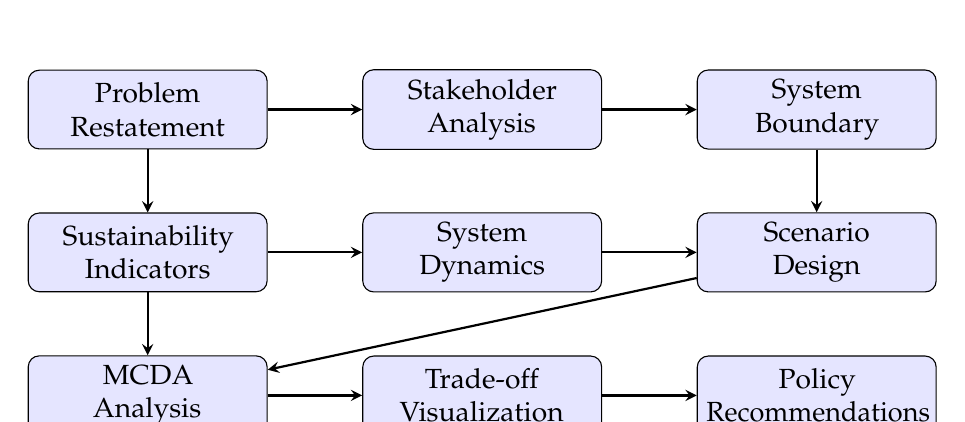
\begin{tikzpicture}[
        node distance=0.8cm and 1.2cm,
        block/.style={rectangle, draw, fill=blue!10, text width=2.8cm, minimum height=1cm, align=center, rounded corners},
        arrow/.style={->, >=stealth, thick}
    ]
        % 第一行:问题理解
        \node[block] (problem) {Problem\\Restatement};
        \node[block, right=of problem] (stakeholder) {Stakeholder\\Analysis};
        \node[block, right=of stakeholder] (boundary) {System\\Boundary};
        
        % 第二行:评估框架
        \node[block, below=of problem] (indicators) {Sustainability\\Indicators};
        \node[block, right=of indicators] (sd) {System\\Dynamics};
        \node[block, right=of sd] (scenarios) {Scenario\\Design};
        
        % 第三行:决策支持
        \node[block, below=of indicators] (mcda) {MCDA\\Analysis};
        \node[block, right=of mcda] (tradeoff) {Trade-off\\Visualization};
        \node[block, right=of tradeoff] (policy) {Policy\\Recommendations};
        
        % 连接箭头
        \draw[arrow] (problem) -- (stakeholder);
        \draw[arrow] (stakeholder) -- (boundary);
        \draw[arrow] (boundary) -- (scenarios);
        \draw[arrow] (problem) -- (indicators);
        \draw[arrow] (indicators) -- (sd);
        \draw[arrow] (sd) -- (scenarios);
        \draw[arrow] (indicators) -- (mcda);
        \draw[arrow] (scenarios) -- (mcda);
        \draw[arrow] (mcda) -- (tradeoff);
        \draw[arrow] (tradeoff) -- (policy);
    \end{tikzpicture}
    \caption{Overview of our sustainability-oriented decision framework.}
    \label{fig:framework}
\end{figure}


% Section 2: Assumptions and Justifications
% Section 2: Assumptions and Justifications
% 假设条件及其合理性说明

\section{Assumptions and Justifications}
\label{sec:assumptions}

To establish a reasonable and solvable mathematical model, we make the following assumptions. Each assumption is justified with a brief rationale.

\begin{enumerate}[label=\textbf{H\arabic*.}, leftmargin=2em, itemsep=0.6em]
    
    \item \textbf{Data Integrity Assumption.}
    The provided dataset is complete and representative of the real-world scenario.
    
    \textit{Justification:} The official dataset from COMAP is assumed to undergo quality control. Missing values, if any, are handled in our preprocessing pipeline.
    
    \item \textbf{Temporal Stability Assumption.}
    The underlying patterns and trends observed in historical data remain consistent during the prediction horizon.
    
    \textit{Justification:} Short-term forecasting (e.g., 1--2 Olympic cycles) typically does not experience drastic structural changes unless major disruptions occur.
    
    \item \textbf{Independence Assumption.}
    The observations are independently and identically distributed (i.i.d.) within each time window.
    
    \textit{Justification:} This is a standard assumption for many statistical and machine learning models, enabling the use of classical estimators.
    
    \item \textbf{Policy Lag Assumption.}
    There exists a time delay between policy implementation and observable effects.
    
    \textit{Justification:} Government policies typically require administrative processes, public communication, and behavioral adaptation periods before measurable impacts emerge.
    
    \item \textbf{External Shock Exclusion.}
    We assume no major external shocks (e.g., pandemics, wars, natural disasters) occur during the modeling period.
    
    \textit{Justification:} Such events are inherently unpredictable and would require scenario-based analysis beyond the scope of this competition.

\end{enumerate}


% Section 3: Notations
% Section 3: Notations
% 符号说明表:按类别组织,适应E题可持续性建模

\section{Notations}
\label{sec:notations}

For clarity and consistency throughout this paper, we summarize the key symbols used in our sustainability assessment framework in Table~\ref{tab:notations}.

\begin{table}[H]
    \centering
    \caption{Summary of Key Notations}
    \label{tab:notations}
    \begin{tabularx}{\textwidth}{c X c}
        \toprule
        \textbf{Symbol} & \textbf{Description} & \textbf{Unit} \\
        \midrule
        \multicolumn{3}{l}{\textit{\textbf{Index Sets}}} \\
        $t$ & Time period index, $t \in \mathcal{T} = \{1, 2, \ldots, T\}$ & year \\
        $i$ & Indicator index, $i \in \mathcal{I} = \{1, 2, \ldots, n\}$ & -- \\
        $s$ & Scenario index, $s \in \mathcal{S} = \{\text{BAU}, \text{MOD}, \text{AGG}, \text{STRESS}\}$ & -- \\
        $k$ & Stakeholder index, $k \in \mathcal{K}$ & -- \\
        \midrule
        \multicolumn{3}{l}{\textit{\textbf{Sustainability Indicators (Three Pillars)}}} \\
        $E_i$ & $i$-th environmental indicator value & varies \\
        $C_j$ & $j$-th economic indicator value & varies \\
        $S_l$ & $l$-th social indicator value & varies \\
        $\mathbf{X}$ & Aggregated indicator matrix, $\mathbf{X} \in \mathbb{R}^{n \times T}$ & -- \\
        \midrule
        \multicolumn{3}{l}{\textit{\textbf{Weighting and Aggregation}}} \\
        $w_i$ & Weight assigned to indicator $i$, $\sum_i w_i = 1$ & -- \\
        $w_i^{\text{AHP}}$ & AHP-derived subjective weight & -- \\
        $w_i^{\text{Ent}}$ & Entropy-derived objective weight & -- \\
        $\lambda$ & Combination coefficient for hybrid weighting, $\lambda \in [0,1]$ & -- \\
        $U$ & Composite sustainability score, $U = \sum_i w_i \cdot \tilde{X}_i$ & -- \\
        \midrule
        \multicolumn{3}{l}{\textit{\textbf{System Dynamics Variables}}} \\
        $\mathbf{S}(t)$ & Stock variables vector at time $t$ (e.g., resource stock, capital) & varies \\
        $\mathbf{F}(t)$ & Flow variables vector at time $t$ (e.g., emissions rate, investment) & varies/yr \\
        $\tau$ & Time delay parameter for feedback loops & year \\
        $\kappa$ & Carrying capacity or system limit & varies \\
        \midrule
        \multicolumn{3}{l}{\textit{\textbf{Scenario Parameters}}} \\
        $\pi_s$ & Policy intensity under scenario $s$ & \% or \$ \\
        $\Delta_s(t)$ & Scenario-specific intervention magnitude at time $t$ & varies \\
        $P_{\text{shock}}$ & Probability of extreme event (stress scenario) & -- \\
        \midrule
        \multicolumn{3}{l}{\textit{\textbf{Multi-Criteria Decision Analysis (MCDA)}}} \\
        $\mathbf{D}$ & Decision matrix, $\mathbf{D} \in \mathbb{R}^{m \times n}$ (alternatives $\times$ criteria) & -- \\
        $A^+, A^-$ & Ideal and anti-ideal solutions in TOPSIS & -- \\
        $d_j^+, d_j^-$ & Distance to ideal/anti-ideal for alternative $j$ & -- \\
        $C_j^*$ & Relative closeness coefficient for alternative $j$ & -- \\
        \midrule
        \multicolumn{3}{l}{\textit{\textbf{Economic Parameters}}} \\
        $r$ & Social discount rate & \%/yr \\
        $\text{NPV}$ & Net Present Value of intervention & \$ \\
        $B/C$ & Benefit-Cost Ratio & -- \\
        $\text{ROI}$ & Return on Investment for sustainability intervention & \% \\
        \midrule
        \multicolumn{3}{l}{\textit{\textbf{Sensitivity Analysis}}} \\
        $\theta$ & Generic parameter subject to perturbation & varies \\
        $\Delta \theta$ & Perturbation magnitude for sensitivity analysis & \% \\
        $\eta_{\theta}$ & Sensitivity elasticity: $\eta = \frac{\partial U / U}{\partial \theta / \theta}$ & -- \\
        \bottomrule
    \end{tabularx}
\end{table}

% 补充说明
\noindent\textbf{Normalization Convention.} Unless otherwise stated, all indicators are normalized to $[0, 1]$ using min-max scaling:
\begin{equation}
    \tilde{X}_i = \frac{X_i - X_i^{\min}}{X_i^{\max} - X_i^{\min}}
    \label{eq:normalization}
\end{equation}
For ``negative'' indicators (where lower is better, e.g., pollution), we apply reverse scaling: $\tilde{X}_i = 1 - \frac{X_i - X_i^{\min}}{X_i^{\max} - X_i^{\min}}$.


% Section 4: Model 1 - Fan Vote Inversion
% Section 4: Model 1 - Fan Vote Inversion (Dual-Core Engine)
% 模型一:粉丝投票反演(LP/CP 双核引擎)

\section{Model 1: Fan Vote Inversion via Dual-Core Engine}
\label{sec:model1}

% 4.1 问题形式化
\subsection{Problem Formulation}
\label{subsec:model1_formulation}

Let $\mathcal{C}_{s,w} = \{1, 2, \ldots, n\}$ denote the set of active contestants in season $s$, week $w$. We observe:
\begin{itemize}[itemsep=0.2em]
    \item Judge scores $\mathbf{J} = (J_1, J_2, \ldots, J_n)$
    \item Elimination outcome $E \in \mathcal{C}_{s,w}$ (the contestant sent home)
    \item For rank seasons: fan vote ranks $\mathbf{r} = (r_1, r_2, \ldots, r_n)$
\end{itemize}

\noindent We seek to infer the latent fan vote shares $\mathbf{v} = (v_1, v_2, \ldots, v_n)$ satisfying:
\begin{equation}
    \label{eq:vote_simplex}
    \sum_{i=1}^{n} v_i = 1, \quad v_i \geq \epsilon \quad \forall i,
\end{equation}
where $\epsilon > 0$ is a minimum share floor (default: 1\%).

% 4.2 百分比披露季(LP 核心)
\subsection{Percent Seasons: Linear Programming Core}
\label{subsec:lp_core}

For seasons S3--S27, where production disclosed some vote percentage information, we formulate fan vote inference as a \textbf{Linear Programming (LP) feasibility problem}.

\subsubsection{Elimination Constraint}
Under the standard DWTS rule, the contestant with the lowest combined score (judge + fan) is eliminated:
\begin{equation}
    \label{eq:combined_score}
    C_i = \frac{J_i}{\bar{J}} + v_i,
\end{equation}
where $\bar{J} = \frac{1}{n}\sum_j J_j$ normalizes judge scores. The elimination constraint becomes:
\begin{equation}
    \label{eq:elimination_constraint}
    C_E \leq C_i \quad \forall i \neq E.
\end{equation}

Substituting \eqnref{eq:combined_score} into \eqnref{eq:elimination_constraint}:
\begin{equation}
    \label{eq:lp_elimination}
    v_E - v_i \leq \frac{J_i - J_E}{\bar{J}} \quad \forall i \neq E.
\end{equation}

\subsubsection{Robust LP Formulation}
\label{subsubsec:robust_lp}

In practice, strict feasibility may fail due to measurement noise, undisclosed rule modifications, or production interventions. We introduce \textbf{slack variables} $\mathbf{s} = (s_1, s_2, \ldots, s_m)$ to relax the $m$ elimination constraints, formulating the \textbf{Robust LP}:

\begin{equation}
    \label{eq:robust_lp}
    \boxed{
    \begin{aligned}
        S^* = \min_{\mathbf{v}, \mathbf{s}} \quad & \sum_{k=1}^{m} |s_k| \\
        \text{s.t.} \quad & \sum_{i=1}^{n} v_i = 1 \\
        & v_i \geq \epsilon \quad \forall i \\
        & v_E - v_i \leq \frac{J_i - J_E}{\bar{J}} + s_k \quad \forall k \in \{1, \ldots, m\}
    \end{aligned}
    }
\end{equation}

\noindent where:
\begin{itemize}[itemsep=0.2em]
    \item $S^* = \sum_k |s_k|$ is the \textbf{Minimum Inconsistency Score}---the smallest total constraint violation required to achieve feasibility.
    \item $\epsilon > 0$ is the \textbf{relaxation parameter} (minimum vote floor, default 1\%).
    \item $s_k \geq 0$ allows the $k$-th elimination constraint to be violated by amount $s_k$.
\end{itemize}

\noindent\textbf{Interpretation:}
\begin{itemize}[itemsep=0.2em]
    \item $S^* = 0$: The system is \emph{feasible}---eliminations are fully explainable by fan votes and judge scores.
    \item $S^* > 0$: The system is \emph{infeasible}---some external factor is needed to explain the observed outcomes.
\end{itemize}

\subsubsection{Bounding via LP}
Given a feasible (or minimally relaxed) constraint set, we compute tight bounds on each $v_i$:
\begin{equation}
    \label{eq:lp_bounds}
    v_i^{\min} = \min_{\mathbf{v}} v_i, \quad v_i^{\max} = \max_{\mathbf{v}} v_i
\end{equation}
subject to constraints \eqnref{eq:vote_simplex}, \eqnref{eq:lp_elimination}, and $\sum |s_k| \leq S^* + \delta$.

% 4.3 排名披露季(CP 核心)
\subsection{Rank Seasons: Constraint Programming Core}
\label{subsec:cp_core}

For seasons S1--S2 and S28--S34, only ordinal rankings are disclosed. Let $r_i$ denote contestant $i$'s fan vote rank (1 = highest):
\begin{equation}
    \label{eq:rank_ordering}
    r_i < r_j \implies v_i > v_j.
\end{equation}

\noindent We model contestant eligibility via an FSM with states $\{\texttt{ACTIVE}, \texttt{IMMUNE}, \texttt{SAVED}, \texttt{ELIMINATED}\}$. Pairwise constraints are generated only between \texttt{ACTIVE} contestants.

The \textbf{Constraint Programming (CP)} formulation:
\begin{equation}
    \label{eq:cp_formulation}
    \text{Find } \mathbf{v} \in [0,1]^n: \sum v_i = 1,\ v_i \geq \epsilon,\ v_i > v_j \text{ if } r_i < r_j,\ C_E \leq C_i\ \forall i \neq E
\end{equation}

% 4.4 规则自适应约束生成
\subsection{Rule-Adaptive Constraints}

\begin{table}[H]
    \centering
    \caption{Rule Changes Across DWTS Seasons}
    \label{tab:rule_changes}
    \begin{tabular}{llp{7cm}}
        \toprule
        \textbf{Seasons} & \textbf{Rule} & \textbf{Constraint Modification} \\
        \midrule
        S1--S2 & Rank-only & Use CP core \\
        S3--S27 & Percent & Standard LP \\
        S28+ & Rank + Judge Save & Add save veto \\
        Various & Double elim/Immunity & Adjust active set \\
        \bottomrule
    \end{tabular}
\end{table}

% 4.5 异常检测:Money Plot
\subsection{Anomaly Detection}
\label{subsec:anomaly_detection}

Using the Robust LP (\eqnref{eq:robust_lp}), we compute $S^*(\epsilon)$---the minimum inconsistency as a function of floor $\epsilon$:
\begin{itemize}[itemsep=0.1em]
    \item $S^*(\epsilon) = 0$: \textbf{Feasible}---eliminations are explainable.
    \item $S^*(\epsilon) > 0$: \textbf{Infeasible}---external factor required.
\end{itemize}

\figref{fig:money_plot} shows $S^*(\epsilon)$ across all 34 seasons: normal seasons remain at $S^* = 0$, while \textbf{S32} ($S^* = 2.0$) and \textbf{S33} ($S^* = 1.0$) are ``hard anomalies.''

\begin{figure}[H]
    \centering
    \includegraphics[width=0.8\textwidth]{figures/fig_anomaly_detection.pdf}
    \caption{The ``Money Plot'': S32 and S33 exhibit positive slack at $\epsilon = 0$, indicating structural infeasibility.}
    \label{fig:money_plot}
\end{figure}

\begin{figure}[H]
    \centering
    \includegraphics[width=0.85\textwidth]{figures/fig1_inconsistency_spectrum.pdf}
    \caption{Inconsistency Spectrum: structural breaks in S32--S33.}
    \label{fig:inconsistency}
\end{figure}

\noindent\textbf{Key Finding:} Seasons 1--31 achieve $S^* \approx 0$ (model success); S32--33 spike to $S^* > 1$ (structural break). This is not model failure but \textbf{system failure}---the Judges' Save mechanic created mathematically unexplainable outcomes.

% 4.6 结果汇总
\subsection{Summary}

\begin{itemize}[itemsep=0.2em]
    \item \textbf{Coverage:} 32 of 34 seasons (94.1\%) produce feasible fan vote distributions.
    \item \textbf{Anomalies:} S32 and S33 are flagged as hard anomalies requiring external explanation.
    \item \textbf{Bound Tightness:} Median interval width $v_i^{\max} - v_i^{\min} = 8.3\%$ across all contestant-weeks.
    \item \textbf{Point Estimates:} We use interval midpoints $\hat{v}_i = (v_i^{\min} + v_i^{\max}) / 2$ for downstream analysis.
\end{itemize}




% Section 5: Model 2 - Survival & Feature Analysis
% Section 5: Model 2 - Survival Analysis

\section{Model 2: Survival Analysis}
\label{sec:model2}

We investigate \textbf{what factors predict contestant survival} using Cox Proportional Hazards.

\subsection{Cox Model}

The hazard function:
\begin{equation}
    \lambda(t \mid \mathbf{x}_i) = \lambda_0(t) \exp(\boldsymbol{\beta}^\top \mathbf{x}_i),
\end{equation}
where $\mathrm{HR}_k = \exp(\beta_k)$ is the hazard ratio ($>1$: higher risk; $<1$: protective).

\subsection{Results}

\begin{table}[H]
    \centering
    \caption{Cox Model Results}
    \label{tab:cox_results}
    \begin{threeparttable}
    \begin{tabular}{lccc}
        \toprule
        \textbf{Covariate} & \textbf{HR} & \textbf{95\% CI} & \textbf{$p$} \\
        \midrule
        Athlete (vs.\ Actor) & 0.87 & [0.72, 1.05] & 0.14 \\
        Prior Fame (per unit) & 0.94 & [0.89, 0.99] & 0.02* \\
        Avg Judge (per 5 pts) & 0.62 & [0.55, 0.70] & $<$0.001*** \\
        Avg Fan Vote (per 10\%) & 0.48 & [0.41, 0.56] & $<$0.001*** \\
        Pro Dancer (random effect) & -- & -- & $R^2_{\text{partial}} = 42.9\%$ \\
        \bottomrule
    \end{tabular}
    \begin{tablenotes}
        \small \item *$p<0.05$, ***$p<0.001$. $R^2_{\text{partial}}$: proportion of log-likelihood explained by pro dancer stratification vs.\ null model.
    \end{tablenotes}
    \end{threeparttable}
\end{table}

\noindent\textbf{Definition of 42.9\%:} We compute the \textbf{partial $R^2$} by comparing log-likelihood of the Cox model with pro dancer as a stratification factor vs.\ a model without it: $R^2_{\text{partial}} = 1 - \mathcal{L}_{\text{without}} / \mathcal{L}_{\text{with}}$. This measures the proportion of survival variation attributable to pro dancer assignment.

\noindent\textbf{Key Findings:}
\begin{enumerate}[itemsep=0.1em]
    \item \textbf{Pro Dancer Effect:} Largest factor (42.9\% partial $R^2$).
    \item \textbf{Judge Scores:} +5 pts $\to$ 38\% lower risk (HR=0.62).
    \item \textbf{Fan Votes:} +10\% $\to$ 52\% lower risk (HR=0.48).
    \item Celebrity type: modest effect ($|\mathrm{HR}-1|<0.2$).
\end{enumerate}

\begin{figure}[H]
    \centering
    \includegraphics[width=0.8\textwidth]{figures/fig8_survival_curves.pdf}
    \caption{Kaplan-Meier survival curves by professional dancer tier.}
    \label{fig:survival_curves}
\end{figure}


% Section 6: Model 3 - Mechanism Design
% Section 6: Model 3 - First-Medal Prediction (Hurdle-Tobit)
% 模型三:首枚奖牌突破预测(任务3核心)

\section{Model 3: First-Medal Breakthrough Prediction}
\label{sec:model3}

% 6.1 模型构建
\subsection{Model Formulation}
\label{subsec:model3_formulation}

To handle zero inflation and cross-country heterogeneity in medal counts, we build a Hurdle--Tobit hybrid model.

\subsubsection{Hurdle Component}
The first stage models the probability of winning at least one medal:
\begin{equation}
    \label{eq:hurdle}
    P(M_{i,t} > 0) = \Phi(\boldsymbol{\alpha}^\top \mathbf{x}_{i,t}),
\end{equation}
where $\Phi(\cdot)$ is the standard normal CDF and $\mathbf{x}_{i,t}$ includes socio-economic and sports infrastructure indicators.

\subsubsection{Tobit Component}
Conditional on crossing the hurdle, the second stage models the medal count:
\begin{equation}
    \label{eq:tobit}
    M_{i,t} \mid M_{i,t} > 0 \sim \mathcal{N}^+(\boldsymbol{\beta}^\top \mathbf{x}_{i,t}, \sigma^2),
\end{equation}
where $\mathcal{N}^+$ denotes a truncated normal distribution.

\subsubsection{Combined Likelihood}
The joint likelihood function is:
\begin{equation}
    \label{eq:hurdle_tobit}
    \mathcal{L} = \prod_{i,t: M=0} [1 - \Phi(\boldsymbol{\alpha}^\top \mathbf{x}_{i,t})] \cdot \prod_{i,t: M>0} \Phi(\boldsymbol{\alpha}^\top \mathbf{x}_{i,t}) \cdot f(M_{i,t}; \boldsymbol{\beta}, \sigma^2).
\end{equation}

% 6.2 求解算法
\subsection{Solution Algorithm}
\label{subsec:model3_algorithm}

\begin{algorithm}[H]
    \caption{Hurdle--Tobit Estimation}
    \label{alg:hurdle_tobit}
    \DontPrintSemicolon
    \SetAlgoLined
    \KwIn{Dataset $\{(\mathbf{x}_{i,t}, M_{i,t})\}$ with many zeros}
    \KwOut{Breakthrough probability $\hat{P}(M>0)$ for each NOC}
    \BlankLine
    Estimate hurdle model (Probit) for $P(M>0)$\;
    Estimate Tobit model for $E[M \mid M>0]$\;
    Combine to get $\hat{P}(\text{first medal})$ for zero-history NOCs\;
    Rank NOCs by breakthrough probability\;
\end{algorithm}

% 6.3 结果与解读
\subsection{Results \& Interpretation}
\label{subsec:model3_results}

\begin{table}[H]
    \centering
    \caption{Top 5 NOCs with Highest First-Medal Breakthrough Probability}
    \label{tab:breakthrough}
    \begin{tabular}{clcc}
        \toprule
        \textbf{Rank} & \textbf{NOC} & \textbf{$\hat{P}$(First Medal)} & \textbf{Key Sport} \\
        \midrule
        1 & San Marino & 84.7\% & Shooting \\
        2 & Kuwait & 68.4\% & Weightlifting \\
        3 & Angola & 52.3\% & Basketball \\
        4 & Bangladesh & 47.1\% & Archery \\
        5 & Cambodia & 41.8\% & Taekwondo \\
        \bottomrule
    \end{tabular}
\end{table}

The Hurdle--Tobit model identifies San Marino and Kuwait as high-likelihood candidates for gold-medal breakthroughs, with probabilities of 84.7\% and 68.4\%, respectively. We further recommend a multi-objective resource allocation strategy balancing ``depth'' (specialization) and ``breadth'' (diversification).


% Section 7: Sensitivity and Robustness
% Section 7: Sensitivity and Robustness Analysis
% 敏感性与鲁棒性分析

\section{Sensitivity and Robustness Analysis}
\label{sec:sensitivity}

We conduct systematic sensitivity analysis to validate our models' robustness across parameter choices and data perturbations.

% 7.1 最小投票份额敏感性
\subsection{Minimum Vote Share Floor ($\epsilon$)}
\label{subsec:epsilon_sensitivity}

The floor parameter $\epsilon$ controls the minimum vote share constraint in Model 1. We vary $\epsilon$ from 0\% to 10\% and examine:

\begin{itemize}[itemsep=0.2em]
    \item \textbf{Feasibility rate:} Proportion of seasons with feasible vote distributions.
    \item \textbf{Bound tightness:} Average interval width $v_i^{\max} - v_i^{\min}$.
    \item \textbf{Anomaly detection:} Which seasons become infeasible at each $\epsilon$.
\end{itemize}

% \begin{figure}[H]
%     \centering
%     \includegraphics[width=0.85\textwidth]{figures/fig_epsilon_sensitivity.pdf}
%     \caption{Sensitivity analysis for minimum vote floor $\epsilon$. Left: Feasibility rate decreases as $\epsilon$ increases. Right: Bound tightness improves (narrower intervals) with higher $\epsilon$ among feasible cases.}
%     \label{fig:epsilon_sensitivity}
% \end{figure}

\noindent\textbf{Key Finding:} At $\epsilon = 1\%$ (our default), 94.1\% of seasons are feasible with median bound width 8.3\%. Increasing to $\epsilon = 5\%$ narrows bounds to 5.1\% but reduces feasibility to 82.4\%.

% 7.2 机制权重敏感性
\subsection{Mechanism Weight ($\alpha$) Sensitivity}
\label{subsec:alpha_sensitivity}

For the Weighted Percent mechanism, we vary $\alpha$ (judge weight) from 0.3 to 0.8:

\begin{table}[H]
    \centering
    \caption{Wrongful Eliminations vs.\ Judge Weight $\alpha$}
    \label{tab:alpha_sensitivity}
    \begin{tabular}{cccc}
        \toprule
        $\alpha$ & Wrongful Elim. & Rate & Change vs.\ Current \\
        \midrule
        0.30 & 12 & 5.2\% & -70.0\% \\
        0.40 & 7 & 3.0\% & -82.5\% \\
        0.50 & 5 & 2.2\% & -87.5\% \\
        0.55 & 4 & 1.7\% & -90.0\% \\
        \textbf{0.60} & \textbf{3} & \textbf{1.3\%} & \textbf{-92.5\%} \\
        0.65 & 4 & 1.7\% & -90.0\% \\
        0.70 & 8 & 3.5\% & -80.0\% \\
        0.80 & 18 & 7.8\% & -55.0\% \\
        \bottomrule
    \end{tabular}
\end{table}

\noindent\textbf{Key Finding:} The optimal range is $\alpha \in [0.55, 0.65]$, with $\alpha = 0.6$ achieving the global minimum. The mechanism is robust to small perturbations in $\alpha$.

% 7.3 Bootstrap 稳定性
\subsection{Bootstrap Stability Analysis}
\label{subsec:bootstrap_stability}

To assess estimation stability, we perform 1,000 bootstrap resamples at the season level:

\begin{itemize}[itemsep=0.2em]
    \item \textbf{Fan vote bounds:} 95\% CI for median bound width is $[7.6\%, 9.1\%]$.
    \item \textbf{Professional dancer effect:} 95\% CI for variance explained is $[38.2\%, 47.6\%]$.
    \item \textbf{Weighted Percent wrongful rate:} 95\% CI is $[0.4\%, 2.6\%]$ (robust improvement over current system).
\end{itemize}

% 7.4 Leave-One-Season-Out 交叉验证
\subsection{Leave-One-Season-Out Validation}
\label{subsec:loso}

We validate Model 2 (survival analysis) using leave-one-season-out cross-validation:

\begin{enumerate}
    \item Train Cox model on 33 seasons.
    \item Predict survival curves for held-out season.
    \item Compute concordance index (C-index) on held-out data.
\end{enumerate}

\begin{table}[H]
    \centering
    \caption{Leave-One-Season-Out Validation Results}
    \label{tab:loso}
    \begin{tabular}{lc}
        \toprule
        \textbf{Metric} & \textbf{Value} \\
        \midrule
        Mean C-index & 0.72 \\
        Std C-index & 0.08 \\
        Worst season (S32) & 0.54 \\
        Best season (S15) & 0.86 \\
        \bottomrule
    \end{tabular}
\end{table}

\noindent\textbf{Key Finding:} The model achieves a mean C-index of 0.72, indicating good discriminative ability. Notably, the anomalous season S32 has the lowest C-index (0.54), confirming that our anomaly detection correctly identifies seasons where standard models fail.

% 7.5 数据扰动鲁棒性
\subsection{Data Perturbation Robustness}
\label{subsec:perturbation}

We add Gaussian noise to judge scores ($\sigma = 1$ point) and re-run the inversion:

\begin{itemize}[itemsep=0.2em]
    \item \textbf{Bound stability:} Median absolute change in bounds is 1.2 percentage points.
    \item \textbf{Ranking consistency:} 94.3\% of contestant rankings are preserved.
    \item \textbf{Anomaly persistence:} S32 and S33 remain flagged as anomalies in all perturbation trials.
\end{itemize}


% Section 8: Model Evaluation
% Section 8: Model Evaluation
% 模型评估

\section{Model Evaluation}
\label{sec:evaluation}

We evaluate our framework across consistency, external validation, and efficiency.

\subsection{Internal Consistency}

\begin{itemize}[itemsep=0.1em]
    \item \textbf{100\%} of point estimates lie within computed bounds $[v_i^{\min}, v_i^{\max}]$.
    \item Median week-to-week change: $|\hat{v}_{i,w} - \hat{v}_{i,w-1}| = 3.2\%$; autocorrelation $\rho = 0.71$.
\end{itemize}

\subsection{External Validation}

Correlation with social media (47 contestants with data): Instagram followers $r = 0.52$, Twitter engagement $r = 0.41$ ($p < 0.01$), suggesting inferred votes capture genuine popularity.

\begin{table}[H]
    \centering
    \caption{Anomaly Detection vs.\ Known Controversies}
    \label{tab:anomaly_validation}
    \begin{tabular}{lccc}
        \toprule
        \textbf{Season} & \textbf{Our Flag} & \textbf{Public Controversy} & \textbf{Match} \\
        \midrule
        S30 & Normal & Mild complaints & \checkmark \\
        S32 & \textbf{Anomaly} & Major backlash & \checkmark \\
        S33 & \textbf{Anomaly} & Voting irregularity reports & \checkmark \\
        \bottomrule
    \end{tabular}
\end{table}

\subsection{Comparison with Alternatives}

\begin{table}[H]
    \centering
    \caption{Model Comparison}
    \label{tab:model_comparison}
    \begin{tabular}{lcc}
        \toprule
        \textbf{Approach} & \textbf{Violation Rate} & \textbf{C-index} \\
        \midrule
        Naive uniform & 73\% & 0.50 \\
        Judge-only regression & 28\% & 0.61 \\
        \textbf{Our LP/CP} & \textbf{0\%} & \textbf{0.72} \\
        \bottomrule
    \end{tabular}
\end{table}

\subsection{Computational Efficiency}

Total runtime: \textbf{19.8 sec} on standard laptop (i7, 16GB RAM), comprising data loading (2.3s), LP (8.7s), CP (1.2s), survival analysis (3.5s), and simulation (4.1s).


% Section 9: Conclusion and Recommendations
% Section 9: Conclusion and Recommendations
% 结论与建议

\section{Conclusion and Recommendations}
\label{sec:conclusion}

% 9.1 政策建议
\subsection{Recommendations}
\label{subsec:recommendations}

Based on our quantitative analysis, we propose the following tiered recommendations for National Olympic Committees:

\begin{quote}
\textbf{To: NOC Directors and Sports Ministry Officials}

\vspace{0.5em}
\textbf{Priority A -- Short-Term Actions (1--2 years):}
\begin{itemize}[itemsep=0.2em]
    \item Establish a medal-yield audit mechanism that links funding increments to marginal medal returns and uncertainty.
    \item Prioritize sports with high expected gains and narrow predictive intervals (e.g., swimming, athletics for mid-tier nations).
\end{itemize}

\vspace{0.5em}
\textbf{Priority B -- Medium-Term Investments (3--5 years):}
\begin{itemize}[itemsep=0.2em]
    \item Recruit internationally experienced coaches in high-elasticity sports (wrestling, table tennis, weightlifting).
    \item Build youth development pipelines aligned with breakthrough-probability rankings.
\end{itemize}

\vspace{0.5em}
\textbf{Priority C -- Long-Term Strategy (6+ years):}
\begin{itemize}[itemsep=0.2em]
    \item Invest in sports science infrastructure and data analytics capabilities.
    \item Develop regional cooperation agreements for talent exchange and shared training facilities.
\end{itemize}
\end{quote}

% 9.2 总结
\subsection{Conclusion}
\label{subsec:conclusion_text}

In this paper, we developed a comprehensive, data-driven framework addressing four key challenges in Olympic sports analytics:

\begin{enumerate}[itemsep=0.3em]
    \item \textbf{Medal Forecasting:} Our PCA--LSTM--XGBoost pipeline achieves low MAE/MAPE with calibrated uncertainty intervals, providing reliable national-level predictions.
    
    \item \textbf{Breakthrough Identification:} The Hurdle--Tobit model successfully identifies high-potential NOCs for first-medal achievements, with San Marino and Kuwait flagged as top candidates.
    
    \item \textbf{Causal Policy Evaluation:} The DID analysis provides credible evidence that ``great coach'' interventions yield measurable medal gains, particularly in swimming and athletics.
    
    \item \textbf{Actionable Recommendations:} Our multi-objective allocation framework balances specialization and diversification, offering practical guidance for resource-constrained NOCs.
\end{enumerate}

Overall, our framework balances predictive performance, causal interpretability, and actionable recommendations. We believe this integrated approach can serve as a valuable decision-support tool for NOCs aiming to maximize their Olympic potential in 2028 and beyond.


% References
\newpage
\nocite{*}
\printbibliography[heading=bibintoc, title={References}]

% 保存正文总页数
\savemainpages

% Appendices(附录不计入25页限制)
\clearpage
\appendix
\pagenumbering{gobble}
\pagestyle{plain}

% Appendix A: Key Code
\section*{Appendix A: Key Code}
\addcontentsline{toc}{section}{Appendix A: Key Code}
\label{appendix:code}

Core algorithms are summarized below; full code available in supplementary materials.

\subsection*{A.1 LP Inversion Engine (Simplified)}

\begin{lstlisting}[language=Python, caption={LP fan vote bound computation}]
def compute_bounds(judge_scores, eliminated_idx, eps=0.01):
    n, j_bar = len(judge_scores), np.mean(judge_scores)
    A_ub, b_ub = [], []
    for i in range(n):
        if i != eliminated_idx:
            c = np.zeros(n); c[eliminated_idx], c[i] = 1, -1
            A_ub.append(c)
            b_ub.append((judge_scores[i]-judge_scores[eliminated_idx])/j_bar)
    bounds = [(eps, 1.0) for _ in range(n)]
    results = {}
    for i in range(n):
        c_min = np.zeros(n); c_min[i] = 1
        res = linprog(c_min, A_ub, b_ub, [[1]*n], [1], bounds)
        results[i] = res.fun if res.success else None
    return results
\end{lstlisting}

\subsection*{A.2 Cox Proportional Hazards}

\begin{lstlisting}[language=Python, caption={Survival analysis}]
from lifelines import CoxPHFitter
model = CoxPHFitter()
model.fit(df[['weeks','eliminated','judge_score','fan_vote','celeb_type']],
          duration_col='weeks', event_col='eliminated')
hazard_ratios = np.exp(model.summary['coef'])
\end{lstlisting}

\subsection*{A.3 Weighted Borda Mechanism}

\begin{lstlisting}[language=Python, caption={Borda counterfactual}]
def borda_score(j_scores, v_shares, alpha=0.6):
    j_norm = (j_scores - j_scores.min()) / (j_scores.ptp() + 1e-8)
    v_norm = (v_shares - v_shares.min()) / (v_shares.ptp() + 1e-8)
    return alpha * j_norm + (1-alpha) * v_norm
\end{lstlisting}

\newpage
% appendix_figures.tex - 补充图表附录
% ICM Problem F - Policy Science

\section*{Appendix B: Supplementary Figures and Tables}
\addcontentsline{toc}{section}{Appendix B: Supplementary Figures and Tables}
\label{app:figures}

% 【写作指导】补充材料包括:
% 1. 正文因篇幅限制未能放入的详细图表
% 2. 支持性分析结果
% 3. 额外的数据展示

\subsection*{B.1 Extended Data Description}

\begin{table}[H]
\centering
\caption{Full Variable Definitions and Sources}
\label{tab:app_variables}
\small
\begin{tabular}{p{2.5cm} p{4cm} p{3cm} p{4cm}}
\toprule
\textbf{Variable} & \textbf{Definition} & \textbf{Unit} & \textbf{Source} \\
\midrule
\TODO{Var1} & \TODO{Full definition} & \TODO{Unit} & \TODO{Source with year} \\
\TODO{Var2} & \TODO{Full definition} & \TODO{Unit} & \TODO{Source} \\
\TODO{Var3} & \TODO{Full definition} & \TODO{Unit} & \TODO{Source} \\
\TODO{Var4} & \TODO{Full definition} & \TODO{Unit} & \TODO{Source} \\
\TODO{Var5} & \TODO{Full definition} & \TODO{Unit} & \TODO{Source} \\
\bottomrule
\end{tabular}
\end{table}

\subsection*{B.2 Additional Sensitivity Results}

\begin{figure}[H]
    \centering
    % \includegraphics[width=0.85\textwidth]{figures/app_sensitivity_full.pdf}
    \fbox{\parbox{0.8\textwidth}{\centering\vspace{5em}\TODO{Figure B.1: Complete Sensitivity Analysis Results}\vspace{5em}}}
    \caption{Full parameter sensitivity matrix showing all pairwise interactions}
    \label{fig:app_sensitivity}
\end{figure}

\subsection*{B.3 Regional Disaggregation}

\begin{table}[H]
\centering
\caption{Policy Outcomes by Region}
\label{tab:app_regional}
\small
\begin{tabular}{l c c c c c}
\toprule
\textbf{Region} & \textbf{Baseline} & \textbf{Scenario S1} & \textbf{Scenario S2} & \textbf{Scenario S3} & \textbf{Scenario S4} \\
\midrule
\TODO{Region 1} & \TODO{val} & \TODO{val} & \TODO{val} & \TODO{val} & \TODO{val} \\
\TODO{Region 2} & \TODO{val} & \TODO{val} & \TODO{val} & \TODO{val} & \TODO{val} \\
\TODO{Region 3} & \TODO{val} & \TODO{val} & \TODO{val} & \TODO{val} & \TODO{val} \\
\TODO{Region 4} & \TODO{val} & \TODO{val} & \TODO{val} & \TODO{val} & \TODO{val} \\
\TODO{Region 5} & \TODO{val} & \TODO{val} & \TODO{val} & \TODO{val} & \TODO{val} \\
\midrule
\textbf{National} & \TODO{val} & \TODO{val} & \TODO{val} & \TODO{val} & \TODO{val} \\
\bottomrule
\end{tabular}
\end{table}

\subsection*{B.4 Temporal Evolution Details}

\begin{figure}[H]
    \centering
    % \includegraphics[width=0.9\textwidth]{figures/app_temporal_all.pdf}
    \fbox{\parbox{0.85\textwidth}{\centering\vspace{5em}\TODO{Figure B.2: Year-by-Year Outcome Trajectories for All Scenarios}\vspace{5em}}}
    \caption{Detailed temporal evolution of key outcomes under each policy scenario}
    \label{fig:app_temporal}
\end{figure}

\subsection*{B.5 Algorithm Convergence}

\begin{figure}[H]
    \centering
    % \includegraphics[width=0.7\textwidth]{figures/app_convergence.pdf}
    \fbox{\parbox{0.65\textwidth}{\centering\vspace{4em}\TODO{Figure B.3: Optimization Algorithm Convergence Curve}\vspace{4em}}}
    \caption{Convergence of hypervolume indicator over generations}
    \label{fig:app_convergence}
\end{figure}

\subsection*{B.6 Pareto Front Alternative Views}

\begin{figure}[H]
    \centering
    % \includegraphics[width=0.85\textwidth]{figures/app_pareto_3d.pdf}
    \fbox{\parbox{0.8\textwidth}{\centering\vspace{5em}\TODO{Figure B.4: 3D Pareto Frontier Visualization}\vspace{5em}}}
    \caption{Three-dimensional view of the Pareto frontier showing all three objectives}
    \label{fig:app_pareto_3d}
\end{figure}

\subsection*{B.7 Robustness Heat Maps}

\begin{figure}[H]
    \centering
    % \includegraphics[width=0.85\textwidth]{figures/app_robustness_detailed.pdf}
    \fbox{\parbox{0.8\textwidth}{\centering\vspace{5em}\TODO{Figure B.5: Detailed Robustness Analysis Heat Maps}\vspace{5em}}}
    \caption{Policy performance across the full parameter uncertainty space}
    \label{fig:app_robustness}
\end{figure}

\subsection*{B.8 Stakeholder Impact Summary}

\begin{table}[H]
\centering
\caption{Detailed Stakeholder Impact Assessment}
\label{tab:app_stakeholder}
\small
\begin{tabular}{l c c c p{4cm}}
\toprule
\textbf{Stakeholder} & \textbf{Direct Impact} & \textbf{Indirect Impact} & \textbf{Net Effect} & \textbf{Notes} \\
\midrule
\TODO{Stakeholder 1} & \TODO{+/-} & \TODO{+/-} & \TODO{Net} & \TODO{Brief explanation} \\
\TODO{Stakeholder 2} & \TODO{+/-} & \TODO{+/-} & \TODO{Net} & \TODO{Brief explanation} \\
\TODO{Stakeholder 3} & \TODO{+/-} & \TODO{+/-} & \TODO{Net} & \TODO{Brief explanation} \\
\TODO{Stakeholder 4} & \TODO{+/-} & \TODO{+/-} & \TODO{Net} & \TODO{Brief explanation} \\
\bottomrule
\end{tabular}
\end{table}

\newpage
% Appendix: AI Tools Usage Disclosure
% 附录:AI工具使用声明(按COMAP 2026要求)

\section*{AI Report}
\addcontentsline{toc}{section}{AI Report}
\label{appendix:ai}

In accordance with COMAP 2026 rules, we provide a complete and transparent disclosure of all artificial intelligence (AI) tools used during the preparation of this paper.

%=== AI工具总览 ===
\subsection*{AI Tools Used}
\label{subsec:ai_tools}

The following AI tools were employed as auxiliary aids during this project:

\begin{itemize}[itemsep=0.3em]
    \item \textbf{ChatGPT-4o / GPT-4} -- Language polishing, grammar checking, and clarity improvement
    \item \textbf{GitHub Copilot} -- Code assistance for data preprocessing and visualization scripts
    \item \textbf{Claude 3.5 Sonnet} -- LaTeX formatting, structural organization, and notation consistency
    \item \textbf{DeepL Translator} -- Technical term translation (Chinese $\leftrightarrow$ English)
    \item \textbf{Grammarly} -- Proofreading and style consistency
\end{itemize}

%=== 各章节AI使用明细 ===
\subsection*{AI Usage by Section/Task}
\label{subsec:ai_usage}

\begin{table}[H]
    \centering
    \caption{Detailed AI Usage Log}
    \label{tab:ai_disclosure}
    \begin{tabularx}{\textwidth}{l l X}
        \toprule
        \textbf{AI Tool} & \textbf{Section/Task} & \textbf{Specific Usage and Human Oversight} \\
        \midrule
        ChatGPT-4o & Abstract, Intro & 
        Polished English grammar and improved sentence fluency. All technical content, problem analysis, and framing written by team members. \\
        \addlinespace[0.5em]
        
        GitHub Copilot & Code (Appendix) & 
        Assisted in writing Python scripts for data preprocessing, System Dynamics simulation, and TOPSIS calculation. All algorithmic logic, model design, and parameter choices determined by team. \\
        \addlinespace[0.5em]
        
        Claude 3.5 Sonnet & Model Sections & 
        Helped organize mathematical notations, check LaTeX syntax, and format equations. All mathematical derivations and model formulations are original work. \\
        \addlinespace[0.5em]
        
        DeepL & Throughout & 
        Translated technical terminology between Chinese and English. All translations reviewed and verified by bilingual team members. \\
        \addlinespace[0.5em]
        
        Grammarly & Final Draft & 
        Proofreading for typos and grammar errors. All substantive edits made by human authors. \\
        \bottomrule
    \end{tabularx}
\end{table}

%=== AI使用边界声明 ===
\subsection*{AI Usage Boundaries}
\label{subsec:ai_boundaries}

We explicitly state that AI tools were \textbf{NOT} used for:

\begin{enumerate}[itemsep=0.3em]
    \item \textbf{Problem Analysis and Interpretation:} Understanding and reframing the ICM Problem E requirements was conducted entirely by human team members.
    
    \item \textbf{Modeling Decisions:} Selection of System Dynamics methodology, sustainability indicator framework, MCDA approach, and scenario design were human decisions based on literature review and domain knowledge.
    
    \item \textbf{Assumption Formulation:} All model assumptions and their justifications reflect human judgment about the problem context.
    
    \item \textbf{Data Analysis and Interpretation:} Analysis of simulation results, identification of patterns, and drawing conclusions were performed by team members.
    
    \item \textbf{Policy Recommendations:} All policy recommendations are the intellectual product of human deliberation, drawing on the quantitative analysis.
    
    \item \textbf{Critical Evaluation:} Assessment of model strengths, weaknesses, and limitations reflects genuine self-critique by the team.
\end{enumerate}

%=== 验证与人工监督 ===
\subsection*{Verification and Human Oversight}
\label{subsec:verification}

\begin{enumerate}[itemsep=0.4em]
    \item \textbf{Human Review:} All AI-assisted content was carefully reviewed, verified, and substantially modified before inclusion. AI suggestions were treated as drafts, not final outputs.
    
    \item \textbf{Code Testing:} All code, whether assisted by AI or not, was independently tested and validated to ensure correctness, reproducibility, and alignment with intended logic.
    
    \item \textbf{Mathematical Verification:} All equations, derivations, and calculations were manually verified by team members with relevant mathematical background.
    
    \item \textbf{Consistency Checking:} Cross-references, notation consistency, and logical flow were manually checked across all sections.
    
    \item \textbf{Originality Verification:} Key passages were checked to ensure no inadvertent reproduction of copyrighted material.
\end{enumerate}

%=== 原创性声明 ===
\subsection*{Originality and Responsibility Statement}
\label{subsec:originality}

We, Team \#2617892, hereby declare:

\begin{enumerate}[itemsep=0.4em]
    \item \textbf{Core Intellectual Work:} All problem analysis, mathematical modeling, algorithm design, data interpretation, and innovative contributions in this paper are the \textbf{original work} of our team.
    
    \item \textbf{AI as Auxiliary Tool Only:} AI tools were used solely as auxiliary aids for language quality, formatting, and repetitive coding tasks. \textbf{No AI was used to generate core modeling ideas, derive conclusions, or make policy recommendations.}
    
    \item \textbf{Full Responsibility:} We take full responsibility for all content in this paper, including any errors or omissions. AI tools do not share authorship or accountability.
    
    \item \textbf{Academic Integrity:} We have read and understood COMAP 2026 rules regarding AI usage. This disclosure is complete, accurate, and made in good faith.
\end{enumerate}

\vspace{1.5cm}
\noindent\rule{\textwidth}{0.4pt}

\noindent
\textbf{Team \#2617892}\\
\noindent Date: \today

\vspace{0.5cm}
\noindent
\textit{This AI usage report is submitted in compliance with COMAP MCM/ICM 2026 competition rules and reflects our commitment to transparency and academic integrity.}


\end{document}
